\documentclass[tikz,border=5pt]{standalone}
\usetikzlibrary{shapes.misc, positioning, calc}

\newcommand{\particle}[5]{
  \node[align = center,
    anchor = #3,
    minimum height = 1.0cm,
    text width = 1.5cm]
  (#1) at (#2)[draw, rounded rectangle]{$#4$\\\tiny#5};
  }
\def\shft{5mm}
\def\sep{10mm}
\usepackage{tikz}
\begin{document}
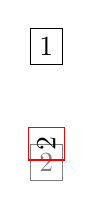
\begin{tikzpicture}
  \node [draw] (first) {1};
  \node [draw, below=of first, opacity=0.5] {2};
    \node [draw=red, below=of first,rotate=90,anchor=center] {2};
  %\node [anchor=center](c)at (0,0){\Huge .};
  %\node [draw, below=of c, rotate=-270, anchor = north](l1) {label1};
  %\node [draw, anchor = north, color = red](l2) at (c.south){label2};
  %\coordinate (D) at  ();
  %\node [align=center](a) [draw, rectangle]{a};
  %\node [align=center, anchor = north](b) at ($(a.south) + (0, -0.3)$) [draw, rectangle]{b};
  %\node [align=center, anchor = west, minimum height=0.5cm, minimum width=0.5cm](c) at ($(a.east) + (0.3, 0)$) \element{c};

\end{tikzpicture}
\end{document}
